\documentclass{article}
\usepackage[a4paper, margin=0.5in, bottom=1.5in]{geometry}
\usepackage{graphicx,xcolor} % Required for inserting images
\usepackage{tabularx}
\usepackage[utf8]{inputenc}
\usepackage[english,spanish]{babel}
\usepackage{titlesec} % Paquete para personalizar los títulos
\usepackage{sectsty} % Paquete para cambiar el estilo de las secciones
\usepackage{tocloft} % Paquete para cambiar el estilo del indice
% Fuente Encode Sans (la que usa Gecko Academy); si no está instalada, Helvetica
\IfFileExists{encodesans.sty}
  {\usepackage[default]{encodesans}}
  {\usepackage{helvet}\renewcommand{\familydefault}{\sfdefault}}
\usepackage{hyperref}
\usepackage{calc}

\usepackage{fancyhdr}
\usepackage[x11names,table,xcdraw]{xcolor}
\usepackage{pgf-pie} % Paquete para gráficos de torta
\usepackage{xcolor}   % Paquete para definir colores
\usepackage{tikz}      % Paquete para gráficos en TikZ
\usepackage{pgfplots}
\usepackage{pgfplotstable}
\usepackage{float}




%Declare custom variables
\newcommand{\brandName}{Matias Nahuel Heredia }
\newcommand{\position}{Information Systems Analyst}
\newcommand{\positiones}{Analista de Sistemas de Información}
\newcommand{\myName}{}
\newcommand{\tab}{\hspace{30pt}}
\newcommand{\typePentest}{Black Box }
\newcommand{\initialDate}{May 12, 2022 }
\newcommand{\finalDate}{May 31, 2022 }
\newcommand{\enterpriseName}{I.N.E }
\newcommand{\documentVersion}{1.0}


\newcommand{\countCritical}{1 }
\newcommand{\countHigh}{2 }
\newcommand{\countMedium}{3 }
\newcommand{\countLow}{4 }
\newcommand{\countInfo}{5 }
\newcommand{\totalCount}{\countCritical+\countHigh+\countMedium+\countLow+\countInfo}

% Declare colors
% Paleta Gecko Academy (academy.binarygecko.com): verde #03A600, verde oscuro #028D00, negro, gris #AAAAAA
\definecolor{geckoGreen}{HTML}{03A600}
\definecolor{geckoGreenDark}{HTML}{028D00}
\definecolor{geckoBlack}{HTML}{000000}
\definecolor{geckoGray}{HTML}{AAAAAA}

\definecolor{topHeaderBackground}{HTML}{000000}
\definecolor{summarySectionColor}{HTML}{03A600}
\definecolor{summarySubsectionColor}{HTML}{028D00}
\definecolor{CriticalVulnColor}{HTML}{d50000}
\definecolor{HighVulnColor}{HTML}{f44336}
\definecolor{MediumVulnColor}{HTML}{e65100}
\definecolor{LowVulnColor}{HTML}{8bc34a}
\definecolor{InfoVulnColor}{HTML}{01579b}
\definecolor{backGroundPageColor}{HTML}{FFFFFF}
\definecolor{textPageColor}{HTML}{111111}



\definecolor{TableHeaderBgRowColor}{HTML}{03A600}
\definecolor{TableBgRowColor}{HTML}{C8EDC7}
\definecolor{TableBgRowIntemediaColor}{HTML}{EEF9EE}

% Enlaces e índice en verde Gecko
\hypersetup{colorlinks=true, linkcolor=geckoGreenDark, urlcolor=geckoGreen, citecolor=geckoGreenDark}
\setlength{\arrayrulewidth}{0.0mm}

% Seccions color's
\sectionfont{\color{summarySectionColor}\sffamily\bfseries}
\subsectionfont{\color{summarySubsectionColor}\sffamily\bfseries}




% table of contents color's
\renewcommand{\cftsecfont}{\color{summarySectionColor}\sffamily\bfseries} 
\renewcommand{\cftsecpagefont}{\color{summarySectionColor}\sffamily\bfseries} 
\renewcommand{\cftsubsecfont}{\color{summarySubsectionColor}\sffamily} 
\renewcommand{\cftsubsecpagefont}{\color{summarySubsectionColor}\sffamily} 
\pagecolor{backGroundPageColor}
\color{textPageColor}




\title{
\iflanguage{english}
{Penetration Test Interno\\ Reporte de vulnerabilidades \\ (Versión:\documentVersion)}
{Internal Penetration Test \\ Report of Findings \\ (Version: \documentVersion)}
}
\author{Matias Nahuel Heredia}
\date{September 2024}


% Configuración de la altura del encabezado
\setlength{\headheight}{30pt} % Aumentar un poco la altura para mayor flexibilidad

% Definición de un estilo de página profesional
\fancypagestyle{professional}{
    \fancyhf{} % Limpiar encabezado y pie de página
    
    % Encabezado izquierdo: Logo
    \fancyhead[L]{%
        
\includegraphics[height=0.8\headheight]{initial/img/gecko-logo.pdf} % Logo ajustado a un 80% de la altura del encabezado
    }
    
    % Encabezado derecho: Título o texto adicional
    \fancyhead[R]{%
        \textbf{\fontsize{12}{14}\selectfont Gecko Academy}\\ % Línea del título
        \textit{\fontsize{10}{12}\selectfont Academy Re-Win -- Entrance Challenge} % Línea del subtítulo
    }
    
    % Línea decorativa debajo del encabezado
    \renewcommand{\headrulewidth}{0.5pt} % Agregar una línea fina
    \renewcommand{\footrulewidth}{0pt}   % Sin línea en el pie de página
}


\begin{document}

% Cambiar el idioma
\selectlanguage{spanish}
% Portada: logo Gecko Academy + título + imagen, todo en la primera página
% (el logo va dentro del título porque \maketitle fuerza un salto de página)
\makeatletter
\let\geckoOrigTitle\@title
\title{%
    {\setlength{\fboxsep}{10pt}\colorbox{black}{
\includegraphics[width=0.55\linewidth]{initial/img/gecko-logo.pdf}}}\\[1.5em]
    \geckoOrigTitle}
\makeatother
\maketitle
\begin{center}
    \includegraphics[width=0.9\linewidth]{initial/img/pentester.jpg}
\end{center}

\newpage
\pagestyle{fancy} % Aplicar encabezado a todas las demás páginas

\tableofcontents
\newpage

\section{\iflanguage{spanish}{Versionado}{Versioning}}
\iflanguage{spanish}
{\begin{center}
\begin{table}[h!]
    \centering
    \begin{tabularx}{\textwidth}{|>{\centering\arraybackslash}m{3cm}|>{\centering\arraybackslash}m{14.5cm}|}
        \hline
        \rowcolor{TableHeaderBgRowColor} 
        \multicolumn{2}{|c|}{\textbf{History Document Versions}} \\
        \hline
        \rowcolor{TableHeaderBgRowColor}
        \textbf{Version} & \textbf{Description} \\
        \hline
        \cellcolor{gray!40}\textcolor{black}{\textbf{1.0}} &
        \cellcolor{gray!40} \textcolor{black}{First Pentesting} \\
        \hline        
    \end{tabularx}
    \label{table:information-security-risk-rating-scale}
\end{table}
\end{center}}
{\begin{center}
\begin{table}[h!]
    \centering
    \begin{tabularx}{\textwidth}{|>{\centering\arraybackslash}m{3cm}|>{\centering\arraybackslash}m{14.5cm}|}
        \hline
        \rowcolor{TableHeaderBgRowColor} 
        \multicolumn{2}{|c|}{\textbf{History Document Versions}} \\
        \hline
        \rowcolor{TableHeaderBgRowColor}
        \textbf{Version} & \textbf{Description} \\
        \hline
        \cellcolor{gray!40}\textcolor{black}{\textbf{1.0}} &
        \cellcolor{gray!40} \textcolor{black}{First Pentesting} \\
        \hline        
    \end{tabularx}
    \label{table:information-security-risk-rating-scale}
\end{table}
\end{center}

}


\section{\iflanguage{spanish}{Contrato de Confidencialidad}{Statement of Confidentiality}}
\iflanguage{spanish}
{{ \tab El contenido de este documento ha sido desarrollado por \brandName. El autor considera que el contenido de este
documento es información confidencial y propietaria de la empresa. Esta información debe ser utilizada únicamente para su propósito previsto.\\
Este documento no puede ser divulgado a otro proveedor, socio comercial o contratista sin el consentimiento previo por escrito de \brandName. Además, ninguna parte de este documento puede ser comunicada, reproducida,
copiada o distribuida sin el consentimiento previo de \brandName.
El contenido de este documento no constituye asesoramiento legal. Los servicios ofrecidos por \brandName relacionados con el cumplimiento, litigios u otros intereses legales no están destinados a ser tomados como asesoramiento jurídico y no deben interpretarse como tal. La evaluación detallada en este documento se refiere a una empresa ficticia con fines de examen, y las vulnerabilidades aquí mencionadas de ninguna manera afectan la infraestructura interna o externa de \enterpriseName. }


}
{
{ \tab The contents of this document have been developed by \brandName. The author considers the contents of this
document to be proprietary and business confidential information. This information is to be used only for its intended purpose.\\This document may not be released to another vendor, business partner, or contractor without prior
written consent from \brandName. Additionally, no portion of this document may be communicated, reproduced,
copied or distributed without the prior consent of \brandName.
The contents of this document do not constitute legal advice. \brandName’s offer of services that relate to compliance,
litigation or other legal interests are not intended as legal counsel and should not be taken as such. The assessment
detailed herein is against a fictional company for exam purposes, and the vulnerabilities in no way
affect \enterpriseName's external or internal infrastructure.}

}


\section{\iflanguage{spanish}{Contactos Involucrados}{Engagement Contacts}}
\iflanguage{spanish}
{\begin{table}[h!]
    \centering
    \begin{tabularx}{\textwidth}{|X|X|X|} 
        \hline
        \rowcolor{TableHeaderBgRowColor} 
        \multicolumn{3}{|c|}{\textbf{Contactos de Inlanefreight}} \\       
        
        \cellcolor{TableBgRowColor} \textbf{Matías Nahuel Heredia} & 
        \cellcolor{TableBgRowColor} \textbf{Analista de Sistemas de Información} & 
        \cellcolor{TableBgRowColor} \textbf{matiasnahuelheredia@gmail.com} \\
        \hline

        %\cellcolor{TableBgRowIntemediaColor} \textbf{Contacto Secundario} & 
        %\cellcolor{TableBgRowIntemediaColor} \textbf{Título} & 
        %\cellcolor{TableBgRowIntemediaColor} \textbf{Correo Electrónico del Contacto Secundario} \\
        %\hline
    \end{tabularx}
    \label{tabla:ancho-completo}
\end{table}

\begin{table}[h!]
    \centering
    \begin{tabularx}{\textwidth}{|X|X|X|} 
        \hline
        \rowcolor{TableHeaderBgRowColor} 
        \multicolumn{3}{|c|}{\textbf{Contacto del Evaluador}} \\       
        
        \cellcolor{TableBgRowColor} \textbf{-} & 
        \cellcolor{TableBgRowColor} \textbf{-} & 
        \cellcolor{TableBgRowColor} \textbf{-} \\
        \hline

        %\cellcolor{TableBgRowIntemediaColor} \textbf{Contacto Secundario} & 
        %\cellcolor{TableBgRowIntemediaColor} \textbf{Título} & 
        %\cellcolor{TableBgRowIntemediaColor} \textbf{Correo Electrónico del Contacto Secundario} \\
        %\hline
    \end{tabularx}
    \label{tabla:ancho-completo}
\end{table}
}
{\begin{table}[h!]
    \centering
    \begin{tabularx}{\textwidth}{|X|X|X|} 
        \hline
        \rowcolor{TableHeaderBgRowColor} 
        \multicolumn{3}{|c|}{\textbf{Inlanefreight Contacts}} \\       
        
        \cellcolor{TableBgRowColor} \textbf{Matias Nahuel Heredia} & 
        \cellcolor{TableBgRowColor} \textbf{Information Systems Analyst} & 
        \cellcolor{TableBgRowColor} \textbf{matiasnahuelheredia@gmail.com} \\
        \hline

        %\cellcolor{TableBgRowIntemediaColor} \textbf{Secondary Contact} & 
        %\cellcolor{TableBgRowIntemediaColor} \textbf{Title} & 
        %\cellcolor{TableBgRowIntemediaColor} \textbf{Secondary Contact Email} \\
        %\hline
    \end{tabularx}
    \label{tabla:ancho-completo}
\end{table}

\begin{table}[h!]
    \centering
    \begin{tabularx}{\textwidth}{|X|X|X|} 
        \hline
        \rowcolor{TableHeaderBgRowColor} 
        \multicolumn{3}{|c|}{\textbf{Assessor Contact}} \\       
        
        \cellcolor{TableBgRowColor} \textbf{-} & 
        \cellcolor{TableBgRowColor} \textbf{-} & 
        \cellcolor{TableBgRowColor} \textbf{-} \\
        \hline

        %\cellcolor{TableBgRowIntemediaColor} \textbf{Secondary Contact} & 
        %\cellcolor{TableBgRowIntemediaColor} \textbf{Title} & 
        %\cellcolor{TableBgRowIntemediaColor} \textbf{Secondary Contact Email} \\
        %\hline
    \end{tabularx}
    \label{tabla:ancho-completo}
\end{table}}


\section{\iflanguage{spanish}{Resumen Ejecutivo}{Executive Summary}}
\iflanguage{spanish}
{\qquad\enterpriseName Ltd. (“\enterpriseName” en adelante) contrató a \brandName para realizar una Prueba de Penetración de Red en la red interna de \enterpriseName con el objetivo de identificar debilidades de seguridad, determinar el impacto para \enterpriseName, documentar todos los hallazgos de manera clara y repetible, y proporcionar recomendaciones de remediación.
}
{\qquad\enterpriseName Ltd. (“\enterpriseName” herein) contracted \brandName to perform a Network Penetration Test of
\enterpriseName’s internally facing network to identify security weaknesses, determine the impact to \enterpriseName,
document all findings in a clear and repeatable manner, and provide remediation recommendations.}

\subsection{\iflanguage{spanish}{Enfoque}{Approach}}
\iflanguage{spanish}
{\qquad\brandName realizó pruebas bajo un enfoque de “\typePentest” desde \initialDate hasta \finalDate, sin credenciales ni conocimiento previo del entorno interno de \enterpriseName, con el objetivo de identificar debilidades desconocidas. Las pruebas se realizaron desde un punto de vista no invasivo con el objetivo de descubrir la mayor cantidad posible de configuraciones erróneas y vulnerabilidades. Las pruebas se llevaron a cabo de forma remota a través de un host que fue aprovisionado específicamente para esta evaluación. Cada debilidad identificada fue documentada e investigada manualmente para determinar las posibilidades de explotación y el potencial de escalamiento. 

\brandName buscó demostrar el impacto total de cada vulnerabilidad, incluyendo el compromiso del dominio interno. Si \brandName lograba obtener un punto de apoyo en la red interna, \enterpriseName permitió realizar pruebas adicionales, incluyendo movimiento lateral y escalamiento de privilegios horizontales/verticales, para demostrar el impacto de un compromiso de la red interna.
}
{\qquad\brandName performed testing under a “\typePentest” approach \initialDate , to \finalDate without
credentials or any advance knowledge of \enterpriseName’s internally facing environment with the goal of identifying
unknown weaknesses. Testing was performed from a non-evasive standpoint with the goal of uncovering as many
misconfigurations and vulnerabilities as possible. Testing was performed remotely via a host that was provisioned
specifically for this assessment. Each weakness identified was documented and manually investigated to determine
exploitation possibilities and escalation potential. \brandName sought to demonstrate the full impact of every
vulnerability, up to and including internal domain compromise. If \brandName were able to gain a foothold in
the internal network, \enterpriseName allowed for further testing including lateral movement and horizontal/vertical
privilege escalation to demonstrate the impact of an internal network compromise.}

\subsection{\iflanguage{spanish}{Alcance}{Scope}}
\iflanguage{spanish}
{\qquad El alcance de esta evaluación fue un rango de red interna en el dominio \enterpriseName.
}
{\qquad The scope of this assessment was an internal network range in the \enterpriseName domain.}

\subsection{\iflanguage{spanish}{Activos en Alcance}{In-Scope Assets}}
\iflanguage{spanish}
{\begin{table}[h!]
    \centering
    \begin{tabularx}{\textwidth}{|X|X|}
        \hline
        \rowcolor{TableHeaderBgRowColor} 
        \multicolumn{2}{|c|}{\textbf{Activos Dentro del Alcance}} \\
        \hline
        \rowcolor{TableBgRowColor}        
        \textcolor{black}{\textbf{Host/URL/Dirección IP}} &         
        \textcolor{black}{\textbf{Descripción}} \\
        \hline
        \rowcolor{TableBgRowIntemediaColor}        
        \textcolor{black}{\textbf{192.168.195.0/24}} &         
        \textcolor{black}{\textbf{Red interna de Inlanefreight}} \\
        \hline
    \end{tabularx}
    \label{tabla:ancho-completo}
\end{table}
}
{
\begin{table}[h!]
    \centering
    \begin{tabularx}{\textwidth}{|X|X|}
        \hline
        \rowcolor{TableHeaderBgRowColor} 
        \multicolumn{2}{|c|}{\textbf{In-Scope Assets}} \\
        \hline
        \rowcolor{TableBgRowColor}        
        \textcolor{black}{\textbf{Host/URL/IP Address}} &         
        \textcolor{black}{\textbf{Description}} \\
        \hline
        \rowcolor{TableBgRowIntemediaColor}        
        \textcolor{black}{\textbf{192.168.195.0/24}} &         
        \textcolor{black}{\textbf{Inlanefreight internal network}} \\
        \hline
    \end{tabularx}
    \label{tabla:ancho-completo}
\end{table}
}

\subsection{\iflanguage{spanish}{Resumen de Evaluación y Recomendaciones}{Assessment Overview and Recommendations}}
\iflanguage{spanish}
{\qquad Durante la prueba de penetración interna contra \enterpriseName, \brandName identificó \the\numexpr\totalCount\relax hallazgos que
amenazan la confidencialidad, integridad y disponibilidad de los sistemas de información de \enterpriseName. Los hallazgos fueron
clasificados por nivel de gravedad, con \countCritical de los hallazgos asignados con una calificación de riesgo crítico, \countHigh de alto riesgo, \countMedium de riesgo medio, 
\countLow de bajo riesgo y \countInfo de riesgo informativo. También hubo un (1) hallazgo informativo relacionado con la mejora de las capacidades de monitoreo de seguridad dentro de la
red interna.
El evaluador encontró que la gestión de parches y vulnerabilidades de \enterpriseName estaba bien mantenida. Ninguno de los hallazgos en este
informe estuvo relacionado con la falta de parches de sistema operativo o de terceros sobre vulnerabilidades conocidas en servicios y
aplicaciones que podrían resultar en acceso no autorizado y compromiso del sistema. Cada defecto descubierto durante las pruebas estuvo
relacionado con una mala configuración o falta de endurecimiento, siendo la mayoría de ellos problemas de autenticación débil y
autorización débil.
Un hallazgo involucró un protocolo de comunicación de red que puede ser “suplantado” para obtener contraseñas de usuarios internos
que pueden ser utilizadas para obtener acceso no autorizado si un atacante puede acceder a la red sin credenciales. En la mayoría de los entornos corporativos,
este protocolo es innecesario y puede deshabilitarse. Está habilitado por defecto principalmente para pequeñas y medianas empresas que no tienen los recursos para un servidor dedicado de resolución de nombres (el
“directorio telefónico” de su red). Durante la evaluación, se observó la presencia de estos recursos en la
red, por lo que \enterpriseName debería comenzar a formular un plan de pruebas para deshabilitar el servicio peligroso.
El siguiente problema fue una configuración débil relacionada con cuentas de servicio que permite a cualquier usuario autenticado robar un
componente del proceso de autenticación que a menudo puede adivinarse fuera de línea (mediante “cracking” de contraseñas) para revelar la
contraseña del usuario en forma legible. Este tipo de cuentas de servicio suelen tener más privilegios que un
usuario estándar, por lo que obtener una de sus contraseñas en texto claro podría resultar en movimiento lateral o escalada de privilegios
y eventualmente en un compromiso total de la red interna. El evaluador también notó que la misma contraseña se usaba para
el acceso de administrador a todos los servidores dentro de la red interna. Esto significa que si un servidor es comprometido, un atacante
puede reutilizar esta contraseña para acceder a cualquier servidor que la comparta para acceso administrativo. Afortunadamente, ambos problemas pueden corregirse sin la necesidad de herramientas de terceros. Active Directory de Microsoft contiene configuraciones que se pueden utilizar para
minimizar el riesgo de que estos recursos sean explotados en beneficio de usuarios maliciosos.
También se encontró un servidor web ejecutando una aplicación web que usaba credenciales débiles y fácilmente adivinables para acceder a una
consola administrativa que puede ser aprovechada para obtener acceso no autorizado al
servidor subyacente. Esto podría ser
explotado por un atacante en la red interna sin necesidad de una cuenta de usuario válida. Este ataque está muy bien documentado, por lo que es un objetivo muy probable que puede ser particularmente dañino, incluso en manos de un atacante no capacitado.
Idealmente, el acceso externo directo a este servicio debería deshabilitarse, pero si no puede ser, debe reconfigurarse con
credenciales excepcionalmente fuertes que se roten con frecuencia. \enterpriseName también debería considerar maximizar los datos de registro
recopilados desde este dispositivo para garantizar que los ataques contra él puedan ser detectados y triados rápidamente.
El evaluador también encontró carpetas compartidas con permisos excesivos, lo que significa que todos los usuarios en la red interna pueden acceder
a una cantidad considerable de datos. Si bien compartir archivos internamente entre departamentos y usuarios es importante para las operaciones diarias del
negocio, permisos abiertos en las comparticiones de archivos pueden resultar en la divulgación no intencionada de información
confidencial. Incluso si una compartición de archivos no contiene información sensible hoy en día, alguien podría poner allí esos datos sin darse cuenta pensando que están protegidos cuando no lo están. Esta configuración debe cambiarse para garantizar que los usuarios solo puedan acceder a lo necesario para realizar sus tareas diarias.
Finalmente, el evaluador notó que las actividades de prueba parecían pasar desapercibidas, lo que podría representar una oportunidad para
mejorar la visibilidad en la red interna e indica que un atacante real podría permanecer indetectado si se logra acceso interno. \enterpriseName debería crear un plan de remediación basado en la sección Resumen de Remediación de este
informe, abordando todos los hallazgos críticos lo antes posible de acuerdo con las necesidades del negocio. \enterpriseName también debería
considerar realizar evaluaciones periódicas de vulnerabilidades si aún no se están llevando a cabo. Una vez que los problemas
identificados en este informe hayan sido abordados, una evaluación de seguridad más colaborativa y profunda de Active Directory podría
ayudar a identificar oportunidades adicionales para fortalecer el entorno de Active Directory, dificultando el movimiento de los atacantes
por la red y aumentando la probabilidad de que \enterpriseName pueda detectar y responder a
actividad sospechosa.
}
{\qquad During the internal penetration test against \enterpriseName, \brandName identified  \the\numexpr\totalCount\relax findings that
threaten the confidentiality, integrity, and availability of \enterpriseName’s information systems. The findings were
categorized by severity level, with \countCritical of the findings being assigned a critical-risk rating,\countHigh high-risk, \countMedium medium-risk, 
\countLow low risk, and \countInfo info risk. There was also one (1) informational finding related to enhancing security monitoring capabilities within the
internal network.
The tester found \enterpriseName’s patch and vulnerability management to be well-maintained. None of the findings in this
report were related to missing operating system or third-party patches of known vulnerabilities in services and
applications that could result in unauthorized access and system compromise. Each flaw discovered during testing was
related to a misconfiguration or lack of hardening, with most falling under the categories of weak authentication and
weak authorization.
One finding involved a network communication protocol that can be “spoofed” to retrieve passwords for internal users
that can be used to gain unauthorized access if an attacker can gain unauthorized access to the network without
credentials. In most corporate environments, this protocol is unnecessary and can be disabled. It is enabled by default
primarily for small and medium sized businesses that do not have the resources for a dedicated hostname resolution (the
“phonebook” of your network) server. During the assessment, the presence of these resources was observed on the
network, so \enterpriseName should begin formulating a test plan to disable the dangerous service.
The next issue was a weak configuration involving service accounts that allows any authenticated user to steal a
component of the authentication process that can often be guessed offline (via password “cracking”) to reveal the
human-readable form of the account’s password. These types of service accounts typically have more privileges than a
standard user, so obtaining one of their passwords in clear text could result in lateral movement or privilege escalation
and eventually in complete internal network compromise. The tester also noticed that the same password was used for
administrator access to all servers within the internal network. This means that if one server is compromised, an attacker
can re-use this password to access any server that shares it for administrative access. Fortunately, both issues can be
corrected without the need for third-party tools. Microsoft’s Active Directory contains settings that can be used to
minimize the risk of these resources being abused for the benefit of malicious users.
A webserver was also found to be running a web application that used weak and easily guessable credentials to access an
administrative console that can be leveraged to gain unauthorized access to the underlying server. This could be
exploited by an attacker on the internal network without needing a valid user account. This attack is very welldocumented, so it is an exceedingly likely target can be particularly damaging, even in the hands of an unskilled attacker.
Ideally, direct external access to this service would be disabled, but if it cannot be, it should be reconfigured with
exceptionally strong credentials that are rotated frequently. \enterpriseName may also want to consider maximizing the log
data collected from this device to ensure that attacks against it can be detected and triaged quickly.
7
The tester also found shared folders with excessive permissions, meaning that all users in the internal network can access
a considerable amount of data. While sharing files internally between departments and users is important to day-to-day
business operations, wide open permissions on file shares may result in unintentional disclosure of confidential
information. Even if a file share does not contain any sensitive information today, someone may unwittingly put such
data there thinking it is protected when it isn’t. This configuration should be changed to ensure that users can access only
what is necessary to perform their day-to-day duties.
Finally, the tester noticed that testing activities seemed to go mostly unnoticed, which may represent an opportunity to
improve visibility into the internal network and indicates that a real-world attacker might remain undetected if internal
access is achieved. \enterpriseName should create a remediation plan based on the Remediation Summary section of this
report, addressing all high findings as soon as possible according to the needs of the business. \enterpriseName should also
consider performing periodic vulnerability assessments if they are not already being performed. Once the issues
identified in this report have been addressed, a more collaborative, in-depth Active Directory security assessment may
help identify additional opportunities to harden the Active Directory environment, making it more difficult for attackers
to move around the network and increasing the likelihood that \enterpriseName will be able to detect and respond to
suspicious activity}

\section{\iflanguage{spanish}{Resumen de Evaluación de Prueba de Penetración de Red}{Network Penetration Test Assessment Summary}}
\iflanguage{spanish}
{\qquad \brandName comenzó todas las actividades de prueba desde la perspectiva de un usuario no autenticado en la red interna. \enterpriseName proporcionó al evaluador los rangos de red, pero no proporcionó información adicional, como el sistema operativo o información de configuración.
}
{\qquad \brandName began all testing activities from the perspective of an unauthenticated user on the internal
network. \enterpriseName provided the tester with network ranges but did not provide additional information such as
operating system or configuration information. }

\newpage
\subsection{\iflanguage{spanish}{Escala de calificación de riesgos de seguridad de la información}{Information Security Risk Rating Scale}}
\iflanguage{spanish}
{\begin{center}
\begin{table}[h!]
    \centering
    \begin{tabularx}{\textwidth}{|>{\centering\arraybackslash}m{3cm}|>{\centering\arraybackslash}m{3cm}|m{11cm}|}
        \hline
        \rowcolor{TableHeaderBgRowColor} 
        \multicolumn{3}{|c|}{\textbf{Escala de Clasificación de Riesgos de Seguridad de la Información}} \\
        \hline
        \rowcolor{TableHeaderBgRowColor}
        \textbf{Severidad} & \textbf{Puntuación Base} & \textbf{Descripción} \\
        \hline
        \cellcolor{CriticalVulnColor}\textcolor{black}{\textbf{Crítica}} &
        \cellcolor{gray!40} \textcolor{black}{\textbf{9.0 - 10.0}} &
        \cellcolor{gray!40} \textcolor{black}{\textbf{Descripción:} Impacta gravemente la confidencialidad, integridad o disponibilidad de la información, los sistemas o la infraestructura. Permite la explotación de vulnerabilidades críticas que ponen en peligro inmediato la seguridad de la organización.} \\
        \hline
        \cellcolor{HighVulnColor}\textcolor{black}{\textbf{Alta}} &
        \cellcolor{gray!40} \textcolor{black}{\textbf{7.0 - 8.9}} &
        \cellcolor{gray!40} \textcolor{black}{\textbf{Descripción:} Riesgo alto que afecta la seguridad, aunque su explotación no ocurre de forma inmediata. Requiere atención prioritaria para mitigar el riesgo, ya que puede comprometer a la organización si no se aborda adecuadamente.} \\
        \hline
        \cellcolor{MediumVulnColor}\textcolor{black}{\textbf{Media}} &
        \cellcolor{gray!40} \textcolor{black}{\textbf{4.0 - 6.9}} &
        \cellcolor{gray!40} \textcolor{black}{\textbf{Descripción:} Riesgo moderado con impacto potencial en la seguridad. No representa una amenaza inmediata, pero debe ser tratado para evitar que se convierta en un problema más grave.} \\
        \hline
        \cellcolor{LowVulnColor}\textcolor{black}{\textbf{Baja}} &
        \cellcolor{gray!40} \textcolor{black}{\textbf{0.1 - 3.9}} &
        \cellcolor{gray!40} \textcolor{black}{\textbf{Descripción:} Riesgo menor con impacto limitado en la seguridad de la información. Requiere monitoreo, pero no necesita acción urgente.} \\
        \hline
        \cellcolor{InfoVulnColor}\textcolor{black}{\textbf{Informativa}} &
        \cellcolor{gray!40} \textcolor{black}{\textbf{0.0}} &
        \cellcolor{gray!40} \textcolor{black}{\textbf{Descripción:} No representa un riesgo significativo, pero proporciona información útil sobre áreas de mejora potencial o detalles adicionales sobre la infraestructura o configuración.} \\
        \hline
    \end{tabularx}
    \label{table:information-security-risk-rating-scale}
\end{table}
\end{center}
}
{\begin{center}
\begin{table}[h!]
    \centering
    \begin{tabularx}{\textwidth}{|>{\centering\arraybackslash}m{3cm}|>{\centering\arraybackslash}m{3cm}|m{11cm}|}
        \hline
        \rowcolor{TableHeaderBgRowColor} 
        \multicolumn{3}{|c|}{\textbf{Information Security Risk Rating Scale}} \\
        \hline
        \rowcolor{TableHeaderBgRowColor}
        \textbf{Severity} & \textbf{Base Score} & \textbf{Description} \\
        \hline
        \cellcolor{CriticalVulnColor}\textcolor{black}{\textbf{Critical}} &
        \cellcolor{gray!40} \textcolor{black}{\textbf{9.0 - 10.0}} &
        \cellcolor{gray!40} \textcolor{black}{\textbf{Description:} Seriously impacts the confidentiality, integrity, or availability of information, systems, or infrastructure. It can allow exploitation of critical vulnerabilities that immediately jeopardize the security of the organization.} \\
        \hline
        \cellcolor{HighVulnColor}\textcolor{black}{\textbf{High}} &
        \cellcolor{gray!40} \textcolor{black}{\textbf{7.0 - 8.9}} &
        \cellcolor{gray!40} \textcolor{black}{\textbf{Description:} High risk affecting security, although exploitation does not occur immediately. Requires prioritized attention to mitigate the risk, as it can compromise the organization if not properly addressed.} \\
        \hline
        \cellcolor{MediumVulnColor}\textcolor{black}{\textbf{Medium}} &
        \cellcolor{gray!40} \textcolor{black}{\textbf{4.0 - 6.9}} &
        \cellcolor{gray!40} \textcolor{black}{\textbf{Description:} Moderate risk with potential impact on security. It does not pose an immediate threat but must be handled to avoid becoming a more serious problem.} \\
        \hline
        \cellcolor{LowVulnColor}\textcolor{black}{\textbf{Low}} &
        \cellcolor{gray!40} \textcolor{black}{\textbf{0.1 - 3.9}} &
        \cellcolor{gray!40} \textcolor{black}{\textbf{Description:} Minor risk with limited impact on information security. Requires monitoring but does not need urgent action.} \\
        \hline
        \cellcolor{InfoVulnColor}\textcolor{black}{\textbf{Informational}} &
        \cellcolor{gray!40} \textcolor{black}{\textbf{0.0}} &
        \cellcolor{gray!40} \textcolor{black}{\textbf{Description:} Does not represent a significant risk but provides useful information on potential improvement areas or additional details about infrastructure or configuration.} \\
        \hline
    \end{tabularx}
    \label{table:information-security-risk-rating-scale}
\end{table}
\end{center}
}

\subsection{\iflanguage{spanish}{Resumen de Hallazgos}{Summary of Findings}}
\iflanguage{spanish}
{\qquad Durante el curso de la evaluación, \brandName descubrió un total de \the\numexpr\totalCount\relax~hallazgos que representan un riesgo material para los sistemas de información de \enterpriseName. \brandName también identificó un hallazgo informativo que, si se aborda, podría fortalecer aún más la postura general de seguridad de \enterpriseName. Los hallazgos informativos son observaciones sobre áreas de mejora para la organización y no representan vulnerabilidades de seguridad por sí solas. La siguiente tabla proporciona un resumen de los hallazgos clasificados por nivel de severidad.

\begin{table}[h!]
    \centering
    \begin{tabularx}{\textwidth}{|X|X|X|X|X|X|}
        \hline
        \rowcolor{TableHeaderBgRowColor} 
        \multicolumn{6}{|c|}{\textbf{Severidad de los Hallazgos}} \\       
        \hline
        \cellcolor{TableBgRowColor}\centering\textcolor{CriticalVulnColor}{\textbf{Crítico}} & 
        \cellcolor{TableBgRowColor}\centering\textcolor{HighVulnColor}{\textbf{Alto}} &
        \cellcolor{TableBgRowColor}\centering\textcolor{MediumVulnColor}{\textbf{Medio}} &
        \cellcolor{TableBgRowColor}\centering\textcolor{LowVulnColor}{\textbf{Bajo}} &
        \cellcolor{TableBgRowColor}\centering\textcolor{InfoVulnColor}{\textbf{Informativo}} &
        \cellcolor{TableBgRowColor}{\textbf{Total}} \\
        \hline
        \cellcolor{TableBgRowIntemediaColor}\centering\textcolor{CriticalVulnColor}{\textbf{\countCritical}} & 
        \cellcolor{TableBgRowIntemediaColor}\centering\textcolor{HighVulnColor}{\textbf{\countHigh}} &
        \cellcolor{TableBgRowIntemediaColor}\centering\textcolor{MediumVulnColor}{\textbf{\countMedium}} &
        \cellcolor{TableBgRowIntemediaColor}\centering\textcolor{LowVulnColor}{\textbf{\countLow}} &
        \cellcolor{TableBgRowIntemediaColor}\centering\textcolor{InfoVulnColor}{\textbf{\countInfo}} &
        \cellcolor{TableBgRowColor}{
        \textbf{\the\numexpr\totalCount\relax
        }} \\
        \hline
    \end{tabularx}
    \label{tabla:ancho-completo}
\end{table}

\begin{figure}[ht]
\centering
\begin{tikzpicture}
    \pie[
        color={CriticalVulnColor, HighVulnColor, MediumVulnColor, LowVulnColor, InfoVulnColor},
        text=legend, 
        radius=3, 
        sum=auto, 
        radius=3, 
        explode=0.1 
    ]{
        \countCritical/Crítico, % Cantidad de vulnerabilidades críticas
        \countHigh/Alto,     % Cantidad de vulnerabilidades altas
        \countMedium/Medio,   % Cantidad de vulnerabilidades medias
        \countLow/Bajo,      % Cantidad de vulnerabilidades bajas
        \countInfo/Informativo % Cantidad de vulnerabilidades informativas
    }
\end{tikzpicture}
\caption{Distribución de Vulnerabilidades}
\end{figure}
\newpage

A continuación se muestra un resumen de alto nivel de cada hallazgo identificado durante la evaluación. Estos hallazgos se abordan en detalle en la sección de Hallazgos Técnicos del presente informe. 

\begin{table}[h!]
    \centering
    \begin{tabularx}{\textwidth}{|X|X|X|X|}
        \hline
        \rowcolor{TableHeaderBgRowColor}        
        \textcolor{black}{\textbf{\#Hallazgo}} &
        \textcolor{black}{\textbf{Estado}} &
        \textcolor{black}{\textbf{Nivel de Severidad}} &
        \textcolor{black}{\textbf{Nombre del Hallazgo}} \\
        \hline
        \rowcolor{TableBgRowColor}        
        \textcolor{black}{\textbf{2}} &
        \textcolor{black}{\textbf{Nuevo}} &
        \textcolor{HighVulnColor}{\textbf{Alto}} &
        \textcolor{black}{\textbf{Suplantación de Respuesta LLMNR/NBT-NS}} \\
        \hline
        \rowcolor{TableBgRowIntemediaColor}        
        \textcolor{black}{\textbf{1}} &
        \textcolor{black}{\textbf{Nuevo}} &
        \textcolor{LowVulnColor}{\textbf{Bajo}} &
        \textcolor{black}{\textbf{Algo}} \\
        \hline
    \end{tabularx}
    \label{tabla:ancho-completo}
\end{table}
}
{\qquad During the course of testing, \brandName uncovered a total of \the\numexpr\totalCount\relax~findings that pose a material risk to
\enterpriseName’s information systems. \brandName also identified one informational finding that, if addressed,
could further strengthen \enterpriseName’s overall security posture. Informational findings are observations for areas of
improvement by the organization and do not represent security vulnerabilities on their own. The below table provides a
summary of the findings by severity level.


\begin{table}[h!]
    \centering
    \begin{tabularx}{\textwidth}{|X|X|X|X|X|X|}
        \hline
        \rowcolor{TableHeaderBgRowColor} 
        \multicolumn{6}{|c|}{\textbf{Finding Severity}} \\       
        \hline
        \cellcolor{TableBgRowColor}\centering\textcolor{CriticalVulnColor}{\textbf{Critical}} & 
        \cellcolor{TableBgRowColor}\centering\textcolor{HighVulnColor}{\textbf{High}} &
        \cellcolor{TableBgRowColor}\centering\textcolor{MediumVulnColor}{\textbf{Medium}} &
        \cellcolor{TableBgRowColor}\centering\textcolor{LowVulnColor}{\textbf{Low}} &
        \cellcolor{TableBgRowColor}\centering\textcolor{InfoVulnColor}{\textbf{Info}} &
        \cellcolor{TableBgRowColor}{\textbf{Total}} \\
        \hline
        \cellcolor{TableBgRowIntemediaColor}\centering\textcolor{CriticalVulnColor}{\textbf{\countCritical}} & 
        \cellcolor{TableBgRowIntemediaColor}\centering\textcolor{HighVulnColor}{\textbf{\countHigh}} &
        \cellcolor{TableBgRowIntemediaColor}\centering\textcolor{MediumVulnColor}{\textbf{\countMedium}} &
        \cellcolor{TableBgRowIntemediaColor}\centering\textcolor{LowVulnColor}{\textbf{\countLow}} &
        \cellcolor{TableBgRowIntemediaColor}\centering\textcolor{InfoVulnColor}{\textbf{\countInfo}} &
        \cellcolor{TableBgRowColor}{
        \textbf{\the\numexpr\totalCount\relax
        }} \\
        \hline
    \end{tabularx}
    \label{tabla:ancho-completo}
\end{table}

\begin{figure}[ht]
\centering
\begin{tikzpicture}
    \pie[
        color={CriticalVulnColor, HighVulnColor, MediumVulnColor, LowVulnColor, InfoVulnColor},
        text=legend, 
        radius=3, 
        sum=auto, 
        radius=3, 
        explode=0.1 
    ]{
        \countCritical/Critical, % Cantidad de vulnerabilidades críticas
        \countHigh/High,     % Cantidad de vulnerabilidades altas
        \countMedium/Medium,   % Cantidad de vulnerabilidades medias
        \countLow/Low,      % Cantidad de vulnerabilidades bajas
        \countInfo/Info % Cantidad de vulnerabilidades informativas
    }
\end{tikzpicture}
\caption{Vulnerability Distribution}
\end{figure}
\newpage

Below is a high-level overview of each finding identified during testing. These findings are covered in depth in the
Technical Findings Details section of this report. 

\begin{table}[h!]
    \centering
    \begin{tabularx}{\textwidth}{|X|X|X|X|}
        \hline
        \rowcolor{TableHeaderBgRowColor}        
        \textcolor{black}{\textbf{\#Finding}} &
        \textcolor{black}{\textbf{State}} &
        \textcolor{black}{\textbf{Severity Level}} &
        \textcolor{black}{\textbf{Finding Name}} \\
        \hline
        \rowcolor{TableBgRowColor}        
        \textcolor{black}{\textbf{2}} &
        \textcolor{black}{\textbf{New}} &
        \textcolor{HighVulnColor}{\textbf{High}} &
        \textcolor{black}{\textbf{LLMNR/NBT-NS Response Spoofing}} \\
        \hline
        \rowcolor{TableBgRowIntemediaColor}        
        \textcolor{black}{\textbf{1}} &
        \textcolor{black}{\textbf{New}} &
        \textcolor{LowVulnColor}{\textbf{Low}} &
        \textcolor{black}{\textbf{Something}} \\
        \hline
    \end{tabularx}
    \label{tabla:ancho-completo}
\end{table}}

\subsection{\iflanguage{spanish}{Tendencia}{Trends}}
\iflanguage{spanish}
{\begin{figure}[h!]
\centering
\begin{tikzpicture}
    \begin{axis}[
        axis lines=middle,
        symbolic x coords={Audit Version 1, Audit Version 2, Audit Version 3, Audit Version 4},
        xtick=data,
        ylabel={Number of Vulnerabilities},
        xlabel={Audit Versions},
        ymin=0, ymax=10,
        enlarge x limits=0,
        grid=both,
        title={Vulnerability Evolution Across Audit Versions},
        title style={font=\LARGE\bfseries, color=black, align=center, yshift=-1ex},
        ylabel style={font=\small\bfseries, color=black},
        xlabel style={font=\small\bfseries, color=black},
        tick label style={font=\footnotesize, color=black},
        legend style={
            at={(0.5,-0.15)},
            anchor=north,
            legend columns=2,
            font=\small,
            column sep=1ex,
            text=black,
            legend cell align=left
        },
        width=14cm, height=8cm,
        yticklabel style={font=\scriptsize},
        axis line style={draw=black, thick},
        every axis plot/.append style={thick, mark=none, opacity=0.9, color=red},
        % === NUEVO: Fondo para el gráfico ===
        area background/.style={fill=blue!10},
        axis background/.style={fill=blue!10},
    ]

    % Leyenda
    \legend{Critical Vulnerabilities, High Vulnerabilities, Medium Vulnerabilities}

    % Ejemplo de líneas si querés verlas funcionando:
    \addplot coordinates {(Audit Version 1,5) (Audit Version 2,2) (Audit Version 3,2) (Audit Version 4,1)};
     \addplot coordinates {(Audit Version 1,2) (Audit Version 2,1) (Audit Version 3,1) (Audit Version 4,1)};
    \addplot coordinates {(Audit Version 1,1) (Audit Version 2,1) (Audit Version 3,1) (Audit Version 4,8)};

    \end{axis}
\end{tikzpicture}
\caption{Vulnerability Evolution Across Audit Versions (With Trend Lines)}
\end{figure}
}
{\begin{figure}[h!]
\centering
\begin{tikzpicture}
    \begin{axis}[
        axis lines=middle,
        symbolic x coords={Audit Version 1, Audit Version 2, Audit Version 3, Audit Version 4},
        xtick=data,
        ylabel={Number of Vulnerabilities},
        xlabel={Audit Versions},
        ymin=0, ymax=10,
        enlarge x limits=0,
        grid=both,
        title={Vulnerability Evolution Across Audit Versions},
        title style={font=\LARGE\bfseries, color=black, align=center, yshift=-1ex},
        ylabel style={font=\small\bfseries, color=black},
        xlabel style={font=\small\bfseries, color=black},
        tick label style={font=\footnotesize, color=black},
        legend style={
            at={(0.5,-0.15)},
            anchor=north,
            legend columns=2,
            font=\small,
            column sep=1ex,
            text=black,
            legend cell align=left
        },
        width=14cm, height=8cm,
        yticklabel style={font=\scriptsize},
        axis line style={draw=black, thick},
        every axis plot/.append style={thick, mark=none, opacity=0.9, color=red},
        % === NUEVO: Fondo para el gráfico ===
        area background/.style={fill=blue!10},
        axis background/.style={fill=blue!10},
    ]

    % Leyenda
    \legend{Critical Vulnerabilities, High Vulnerabilities, Medium Vulnerabilities}

    % Ejemplo de líneas si querés verlas funcionando:
    \addplot coordinates {(Audit Version 1,5) (Audit Version 2,2) (Audit Version 3,2) (Audit Version 4,1)};
     \addplot coordinates {(Audit Version 1,2) (Audit Version 2,1) (Audit Version 3,1) (Audit Version 4,1)};
    \addplot coordinates {(Audit Version 1,1) (Audit Version 2,1) (Audit Version 3,1) (Audit Version 4,8)};

    \end{axis}
\end{tikzpicture}
\caption{Vulnerability Evolution Across Audit Versions (With Trend Lines)}
\end{figure}
}

\iflanguage{spanish}
{
\begin{figure}[H]
\centering
\begin{tikzpicture}[scale=0.8]

% =========================
% TELARAÑA HEXAGONAL (NIVELES)
% =========================
\foreach \r in {2,4,6,8,10} {
    \draw[gray!40] (0:\r)
        \foreach \a in {60,120,180,240,300} { -- (\a:\r) } -- cycle;
}

% =========================
% EJES RADIALES + ETIQUETAS
% =========================
\foreach \a/\label in {
    0/{Auditoría 1},
    60/{Auditoría 2},
    120/{Auditoría 3},
    180/{Auditoría 4},
    240/{Auditoría 5},
    300/{Auditoría 6}
}{
    \draw[gray!60] (0,0) -- (\a:10);
    \node at (\a:11) {\label};
}

% =========================
% SERIE: VULNERABILIDADES CRÍTICAS
% =========================
\draw[red, thick]
    (0:5) --
    (60:4) --
    (120:3) --
    (180:2) --
    (240:3) --
    (300:4) --
    cycle;

% =========================
% SERIE: VULNERABILIDADES ALTAS
% =========================
\draw[orange, thick]
    (0:3) --
    (60:2) --
    (120:2) --
    (180:1) --
    (240:2) --
    (300:3) --
    cycle;

% =========================
% SERIE: VULNERABILIDADES MEDIAS
% =========================
\draw[blue, thick]
    (0:1) --
    (60:2) --
    (120:2) --
    (180:3) --
    (240:6) --
    (300:4) --
    cycle;

% =========================
% LEYENDA
% =========================
\begin{scope}[shift={(6,-7)}]
    \draw[red, thick] (0,0) -- (1,0);
    \node[right] at (1.2,0) {Vulnerabilidades Críticas};

    \draw[orange, thick] (0,-1) -- (1,-1);
    \node[right] at (1.2,-1) {Vulnerabilidades Altas};

    \draw[blue, thick] (0,-2) -- (1,-2);
    \node[right] at (1.2,-2) {Vulnerabilidades Medias};
\end{scope}

% =========================
% TÍTULO
% =========================
\node[font=\LARGE\bfseries] at (0,13)
{Evolución de Vulnerabilidades – Gráfico de Telaraña Hexagonal};

\end{tikzpicture}
\caption{Comparación de vulnerabilidades mediante gráfico de telaraña hexagonal}
\end{figure}
}
{\centering
\begin{tikzpicture}[scale=0.4]

% =========================
% CÍRCULOS DE REFERENCIA
% =========================
\foreach \r in {2,4,6,8,10} {
    \draw[gray!40] (0,0) circle (\r);
}

% =========================
% EJES RADIALES + ETIQUETAS
% =========================
\foreach \a/\label in {
    0/{Audit Version 1},
    90/{Audit Version 2},
    180/{Audit Version 3},
    270/{Audit Version 4}
}{
    \draw[gray!60] (0,0) -- (\a:10);
    \node at (\a:11) {\label};
}

% =========================
% SERIE: CRITICAL
% =========================
\draw[red, thick]
    (0:5) --
    (90:2) --
    (180:2) --
    (270:1) --
    cycle;

% =========================
% SERIE: HIGH
% =========================
\draw[orange, thick]
    (0:2) --
    (90:1) --
    (180:1) --
    (270:1) --
    cycle;

% =========================
% SERIE: MEDIUM
% =========================
\draw[blue, thick]
    (0:1) --
    (90:1) --
    (180:1) --
    (270:8) --
    cycle;

% =========================
% LEYENDA
% =========================
\begin{scope}[shift={(6,-8)}]
    \draw[red, thick] (0,0) -- (1,0);
    \node[right] at (1.2,0) {Critical Vulnerabilities};

    \draw[orange, thick] (0,-1) -- (1,-1);
    \node[right] at (1.2,-1) {High Vulnerabilities};

    \draw[blue, thick] (0,-2) -- (1,-2);
    \node[right] at (1.2,-2) {Medium Vulnerabilities};
\end{scope}

% =========================
% TÍTULO
% =========================
\node[font=\LARGE\bfseries] at (0,13)
{Vulnerability Evolution Across Audit Versions};

\end{tikzpicture}
\caption{Vulnerability Evolution Across Audit Versions (Radar Chart)}
}


\section{\iflanguage{spanish}{Recorrido de Compromiso de Red Interna}{Internal Network Compromise Walkthrough}}
\iflanguage{spanish}
{\qquad Durante el transcurso de la evaluación, \brandName pudo obtener un acceso inicial y comprometer la red interna, lo que llevó a obtener control administrativo completo sobre el dominio Active Directory \enterpriseName.LOCAL. Los pasos a continuación demuestran el camino tomado desde el acceso inicial hasta el compromiso, y no incluyen todas las vulnerabilidades y configuraciones incorrectas descubiertas durante el proceso de pruebas. Cualquier problema no utilizado como parte del camino hacia el compromiso se enumera como problemas separados e independientes en la sección de Detalles de los Hallazgos Técnicos, clasificados por nivel de severidad. El objetivo de esta cadena de ataque es demostrar a \enterpriseName el impacto de cada vulnerabilidad mostrada en este informe y cómo se conectan entre sí para demostrar el riesgo general para el entorno del cliente y ayudar a priorizar los esfuerzos de remediación (es decir, corregir dos fallos rápidamente podría interrumpir la cadena de ataque mientras la empresa trabaja para remediar todos los problemas reportados). Aunque otros hallazgos mostrados en este informe podrían ser aprovechados para obtener un nivel de acceso similar, esta cadena de ataque muestra el camino inicial de menor resistencia tomado por el evaluador para lograr el compromiso del dominio.
}
{\qquad During the course of the assessment \brandName was able gain a foothold and compromise the internal
network, leading to full administrative control over the \enterpriseName.LOCAL Active Directory domain. The steps
below demonstrate the steps taken from initial access to compromise and does not include all vulnerabilities and
misconfigurations discovered during the course of testing. Any issues not used as part of the path to compromise are
listed as separate, standalone issues in the Technical Findings Details section, ranked by severity level. The intent of this
attack chain is to demonstrate to \enterpriseName the impact of each vulnerability shown in this report and how they fit
together to demonstrate the overall risk to the client environment and help to prioritize remediation efforts (i.e., patching
two flaws quickly could break up the attack chain while the company works to remediate all issues reported). While other
findings shown in this report could be leveraged to gain a similar level of access, this attack chain shows the initial path
of least resistance taken by the tester to achieve domain compromise.
}

\subsection{\iflanguage{spanish}{Recorrido Detallado}{Detailed Walkthrough}}
\iflanguage{spanish}
{---------------------------------
TODO tutorial
---------------------------------

\qquad \brandName realizó las siguientes acciones para comprometer completamente el dominio \enterpriseName.LOCAL.
1. El evaluador utilizó la herramienta Responder para obtener un hash de contraseña NTLMv2 de un usuario del dominio, bsmith.
2. Este hash de contraseña fue descifrado exitosamente fuera de línea usando la herramienta Hashcat, revelando la contraseña en texto claro del usuario, lo que otorgó un punto de acceso al dominio \enterpriseName.LOCAL, pero sin más privilegios que los de un usuario estándar del dominio.
3. Luego, el evaluador ejecutó BloodHound.py, una versión en Python de la popular herramienta de recolección SharpHound, para enumerar el dominio y crear representaciones visuales de las rutas de ataque. Tras una revisión, el evaluador encontró que existían múltiples usuarios privilegiados en el dominio configurados con Service Principal Names (SPNs), los cuales pueden ser aprovechados para realizar un ataque de Kerberoasting y recuperar tickets TGS de Kerberos para las cuentas. Estos tickets pueden ser descifrados fuera de línea usando Hashcat si se ha configurado una contraseña débil. Desde este punto, el evaluador utilizó la herramienta GetUserSPNs.py para realizar un ataque Kerberoasting dirigido contra la cuenta mssqlsvc, encontrando que dicha cuenta tenía derechos de administrador local sobre el host SQL01.\enterpriseName.LOCAL, lo que resultaba un objetivo interesante en el dominio.
4. El evaluador logró descifrar exitosamente la contraseña de esta cuenta fuera de línea, revelando su valor en texto claro.
5. El evaluador pudo autenticarse en el host SQL01.\enterpriseName.LOCAL y recuperar una contraseña en texto claro del registro del host al descifrar secretos LSA para una cuenta (srvadmin) que estaba configurada para inicio de sesión automático.
6. Esta cuenta srvadmin tenía derechos de administrador local sobre todos los servidores (excepto los Controladores de Dominio) en el dominio, por lo que el evaluador pudo iniciar sesión en el host MS01.\enterpriseName.LOCAL y recuperar un ticket TGT de Kerberos para un usuario conectado, pramirez, quien formaba parte del grupo de Administradores de Servidores de Nivel I, otorgándole al evaluador derechos de DCSync sobre el objeto del dominio. Este ataque puede ser utilizado para recuperar el hash de contraseña NTLM de cualquier usuario en el dominio, resultando en el compromiso del dominio y persistencia mediante un Golden Ticket.
7. El evaluador utilizó la herramienta Rubeus para extraer el ticket TGT de Kerberos del usuario pramirez y realizar un ataque de Pass-the-Ticket para autenticarse como este usuario.
8. Finalmente, el evaluador logró realizar un ataque DCSync después de autenticarse exitosamente con esta cuenta de usuario utilizando la herramienta Mimikatz, lo que resultó en el compromiso total del dominio.
}
{---------------------------------
TODO tutorial
---------------------------------


\qquad \brandName performed the following to fully compromise the \enterpriseName.LOCAL domain.
1. The tester utilized the Responder tool to obtain an NTLMv2 password hash for a domain user, bsmith.
2. This password hash was successfully cracked offline using the Hashcat tool to reveal the user's clear text
password which granted a foothold into the \enterpriseName.LOCAL domain, but with no more privileges than
a standard domain user.
3. The tester then ran the BloodHound.py, a Python version of the popular SharpHound collection tool to
enumerate the domain and create visual representations of attack paths. Upon review, the tester found that
multiple privileged users existed in the domain configured with Service Principal Names (SPNs), which can be
leveraged to perform a Kerberoasting attack and retrieve TGS Kerberos tickets for the accounts which can be
cracked offline using Hashcat if a weak password is set. From here, the tester used the GetUserSPNs.py tool to
carry out a targeted Kerberoasting attack against the mssqlsvc account, having found that the mssqlsvc account
had local administrator rights over the host SQL01.\enterpriseName.LOCAL which was an interesting target in
the domain.
4. The tester was able to successfully crack this account's password offline, revealing the clear text value.
5. The tester was able to authenticate to the host SQL01.\enterpriseName.LOCAL and retrieve a clear text
password from the host's registry by decrypting LSA secrets for an account (srvadmin) which was set up for
autologon.
6. This srvadmin account had local administrator rights over all servers (aside from Domain Controllers) in the
domain so the tester was able to log into the MS01.\enterpriseName.LOCAL host and retrieve a Kerberos TGT
ticket for a logged in user, pramirez, who was part of the Tier I Server Admins group which granted the account
DCSync rights over the domain object. This attack can be utilized to retrieve the NTLM password hash for any
user in the domain, resulting in domain compromise and persistence via a Golden Ticket.
7. The tester used the Rubeus tool to extract the Kerberos TGT ticket for the pramirez user and perform a Pass-theTicket attack to authenticate as this user.
8. Finally, the tester was able to perform a DCSync attack after successfully authenticating with this user account
via the Mimikatz tool which ended in domain compromise.

}

%Uncomment this Line
%\section{\iflanguage{spanish}{Incidencias}{Incidents}}
%\iflanguage{spanish}
%{\input{sections/es/incidents}}
%{\input{sections/en/incidents}}


\section{\iflanguage{spanish}{Resumen de Remediación}{Remediation Summary}}
\iflanguage{spanish}
{\qquad Como resultado de esta evaluación, existen varias oportunidades para que \enterpriseName fortalezca la seguridad de su red interna.
Los esfuerzos de remediación se priorizan a continuación, comenzando con aquellos que probablemente tomarán menos tiempo y esfuerzo para
completar. \enterpriseName debe asegurarse de que todos los pasos de remediación y controles mitigantes sean cuidadosamente planificados y probados
para prevenir cualquier interrupción de servicio o pérdida de datos.
}
{\qquad As a result of this assessment there are several opportunities for\enterpriseName to strengthen its internal network security.
Remediation efforts are prioritized below starting with those that will likely take the least amount of time and effort to
complete. \enterpriseName should ensure that all remediation steps and mitigating controls are carefully planned and tested
to prevent any service disruptions or loss of data. }




\subsection{\iflanguage{spanish}{Corto Plazo}{Short Term}}
\iflanguage{spanish}
{\begin{itemize}
\item {[Finding 2] – Establecer contraseñas fuertes (de 24 caracteres o más) en todas las cuentas SPN}
\item {[Finding 5] – Cambiar las credenciales de administrador predeterminadas para el Tomcat Manager}
\item {[Finding 7] – Deshabilitar el listado de directorios en el servidor web afectado}
\item Forzar un cambio de contraseña para todos los usuarios debido al compromiso del dominio
\end{itemize}
}
{\begin{itemize}
\item {[Finding 2] – Set strong (24+ character) passwords on all SPN accounts}
\item .[Finding 5] – Change the default admin credentials for the Tomcat Manager
\item .[Finding 7] – Disable Directory Listing on the affected web server
\item Enforce a password change for all users because of the domain compromise
\end{itemize}}

\subsection{\iflanguage{spanish}{Mediano Plazo}{Medium Term}}
\iflanguage{spanish}
{\begin{itemize}
\item .[Hallazgo 1] – Deshabilitar LLMNR y NBT-NS siempre que sea posible
\item .[Hallazgo 2] – Transicionar de SPNs a Cuentas de Servicio Gestionadas por Grupos (gMSA) siempre que sea posible
\end{itemize}
}
{\begin{itemize}
\item .[Finding 1] – Disable LLMNR and NBT-NS wherever possible
\item .[Finding 2] – Transition from SPNs to Group Managed Service Accounts (gMSA) wherever possible
\end{itemize}
}

\subsection{\iflanguage{spanish}{Largo Plazo}{Long Term}}
\iflanguage{spanish}
{\begin{itemize}
\item Realizar evaluaciones continuas de vulnerabilidades en la red interna y auditorías de contraseñas de dominio
\item Realizar evaluaciones periódicas de seguridad de Active Directory
\item Educar a los administradores de sistemas, redes y desarrolladores sobre las mejores prácticas de endurecimiento de seguridad
\item Mejorar la segmentación de la red para aislar los hosts críticos y limitar los efectos de un compromiso interno
\end{itemize}
}
{\begin{itemize}
\item Perform ongoing internal network vulnerability assessments and domain password audits
\item Perform periodic Active Directory security assessments
\item Educate systems and network administrators and developers on security hardening best practices compromise
\item Enhance network segmentation to isolate critical hosts and limit the effects of an internal compromise
\end{itemize}}

\newpage
\section{\iflanguage{spanish}{Detalles Técnicos de los Hallazgos}{Technical Findings Details}}
\subsection{\iflanguage{spanish}{Detalles}{Details}}

\iflanguage{spanish}
    {{
\begin{table}[h!]
    \centering
    \begin{tabular}{|p{3cm}|p{15cm}|} 
        \hline
        \rowcolor{TableBgRowColor}        
        \cellcolor{HighVulnColor} \textbf{CWE} & 
        \textbf{\href{https://cwe.mitre.org/data/definitions/522.html}{CWE-522} } \\
        \hline
        \rowcolor{TableBgRowIntemediaColor}
        \cellcolor{HighVulnColor} \textbf{Puntuación CVSS 3.1} & 
        \textbf{9.5} \\
        \hline
        \rowcolor{TableBgRowColor}
        \cellcolor{HighVulnColor} \textbf{Impacto} & 
        \textbf{9.5 (AV:N/AC:L/PR:N/UI:N/S:U/C:H/I:H/A:H)} \\
        \hline
        \rowcolor{TableBgRowIntemediaColor}        
        \cellcolor{HighVulnColor} \textbf{Descripción (Incl. Causa Raíz)} & 
        \textbf{Respondiendo al tráfico de red LLMNR/NBT-NS} \\
        \hline        
        \rowcolor{TableBgRowColor}        
        \cellcolor{HighVulnColor} \textbf{Impacto de Seguridad} & 
        \textbf{Los adversarios pueden suplantar una autoridad} \\
        \hline
        \rowcolor{TableBgRowIntemediaColor}        
        \cellcolor{HighVulnColor} \textbf{Dominio Afectado} & 
        \textbf{INLANEFREIGHT.LOCAL} \\
        \hline
        \rowcolor{TableBgRowColor}        
        \cellcolor{HighVulnColor} \textbf{Remediación} & 
        \textbf{
Deshabilitar LLMNR y NetBIOS en la configuración de seguridad del equipo local o mediante políticas de grupo si no son necesarios en el entorno. 
Usar software de seguridad basado en el host para bloquear el tráfico LLMNR/NetBIOS. Habilitar la firma SMB puede detener los ataques de retransmisión NTLMv2. 
Los sistemas de detección y prevención de intrusiones que identifiquen patrones de tráfico indicativos de actividad MiTM pueden mitigar la actividad a nivel de red. 
La segmentación de red puede usarse para aislar componentes de infraestructura que no requieran acceso amplio a la red. Esto puede mitigar, o al menos aliviar, el alcance de la actividad MiTM. 
        } \\
        \hline
        \rowcolor{TableBgRowIntemediaColor}        
        \cellcolor{HighVulnColor} \textbf{Referencias Externas} & 
        \textbf{\url{https://attack.mitre.org/techniques/T1557/001/}} \\
        \hline
    \end{tabular}
\end{table}

% Repetimos para MediumVulnColor
\begin{table}[h!]
    \centering
    \begin{tabular}{|p{3cm}|p{15cm}|} 
        \hline
        \rowcolor{TableBgRowColor}        
        \cellcolor{MediumVulnColor} \textbf{CWE} & 
        \textbf{\href{https://cwe.mitre.org/data/definitions/522.html}{CWE-522} } \\
        \hline
        \rowcolor{TableBgRowIntemediaColor}
        \cellcolor{MediumVulnColor} \textbf{Puntuación CVSS 3.1} & 
        \textbf{9.5} \\
        \hline
        \rowcolor{TableBgRowColor}
        \cellcolor{MediumVulnColor} \textbf{Impacto} & 
        \textbf{9.5 (AV:N/AC:L/PR:N/UI:N/S:U/C:H/I:H/A:H)} \\
        \hline
        \rowcolor{TableBgRowIntemediaColor}        
        \cellcolor{MediumVulnColor} \textbf{Descripción (Incl. Causa Raíz)} & 
        \textbf{Respondiendo al tráfico de red LLMNR/NBT-NS} \\
        \hline        
        \rowcolor{TableBgRowColor}        
        \cellcolor{MediumVulnColor} \textbf{Impacto de Seguridad} & 
        \textbf{Los adversarios pueden suplantar una autoridad} \\
        \hline
        \rowcolor{TableBgRowIntemediaColor}        
        \cellcolor{MediumVulnColor} \textbf{Dominio Afectado} & 
        \textbf{INLANEFREIGHT.LOCAL} \\
        \hline
        \rowcolor{TableBgRowColor}        
        \cellcolor{MediumVulnColor} \textbf{Remediación} & 
        \textbf{(Texto igual que el anterior)} \\
        \hline
        \rowcolor{TableBgRowIntemediaColor}        
        \cellcolor{MediumVulnColor} \textbf{Referencias Externas} & 
        \textbf{\url{https://attack.mitre.org/techniques/T1557/001/}} \\
        \hline
    \end{tabular}
\end{table}

Evidencia de los Hallazgos: \\
\textbf{Ejecutando la herramienta Responder para intentar obtener los hashes de contraseñas de cuentas de usuario.} \\

\begin{figure}[H]
    \centering
    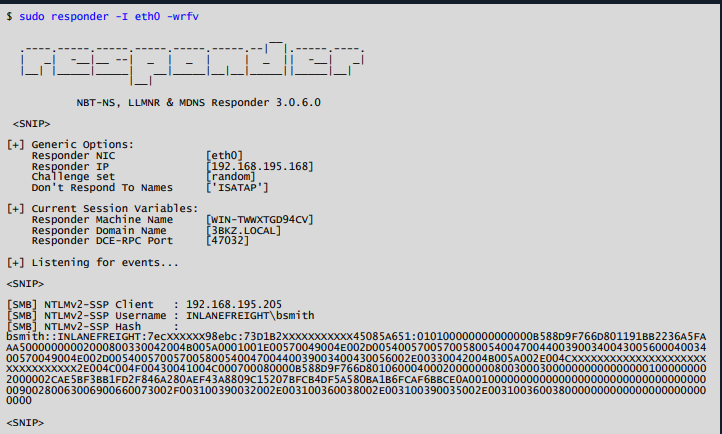
\includegraphics[width=1\linewidth]{initial//evidenceimages/responder.png}
    \caption{Introducir leyenda aquí}
    \label{fig:enter-label}
\end{figure}

\textbf{Descifrado exitoso de un hash de contraseña con Hashcat para revelar el valor en texto claro.}

% Repetimos para LowVulnColor
% Similar estructura que las anteriores tablas.
}
}
    {{
\begin{table}[h!]
    \centering
    \begin{tabular}{|p{3cm}|p{15cm}|} 
        \hline
        \rowcolor{TableBgRowColor}        
        \cellcolor{HighVulnColor} \textbf{CWE} & 
        \textbf{\href{https://cwe.mitre.org/data/definitions/522.html}{CWE-522} } \\
        \hline
        \rowcolor{TableBgRowIntemediaColor}
        \cellcolor{HighVulnColor} \textbf{Puntuación CVSS 3.1} & 
        \textbf{9.5} \\
        \hline
        \rowcolor{TableBgRowColor}
        \cellcolor{HighVulnColor} \textbf{Impacto} & 
        \textbf{9.5 (AV:N/AC:L/PR:N/UI:N/S:U/C:H/I:H/A:H)} \\
        \hline
        \rowcolor{TableBgRowIntemediaColor}        
        \cellcolor{HighVulnColor} \textbf{Descripción (Incl. Causa Raíz)} & 
        \textbf{Respondiendo al tráfico de red LLMNR/NBT-NS} \\
        \hline        
        \rowcolor{TableBgRowColor}        
        \cellcolor{HighVulnColor} \textbf{Impacto de Seguridad} & 
        \textbf{Los adversarios pueden suplantar una autoridad} \\
        \hline
        \rowcolor{TableBgRowIntemediaColor}        
        \cellcolor{HighVulnColor} \textbf{Dominio Afectado} & 
        \textbf{INLANEFREIGHT.LOCAL} \\
        \hline
        \rowcolor{TableBgRowColor}        
        \cellcolor{HighVulnColor} \textbf{Remediación} & 
        \textbf{
Deshabilitar LLMNR y NetBIOS en la configuración de seguridad del equipo local o mediante políticas de grupo si no son necesarios en el entorno. 
Usar software de seguridad basado en el host para bloquear el tráfico LLMNR/NetBIOS. Habilitar la firma SMB puede detener los ataques de retransmisión NTLMv2. 
Los sistemas de detección y prevención de intrusiones que identifiquen patrones de tráfico indicativos de actividad MiTM pueden mitigar la actividad a nivel de red. 
La segmentación de red puede usarse para aislar componentes de infraestructura que no requieran acceso amplio a la red. Esto puede mitigar, o al menos aliviar, el alcance de la actividad MiTM. 
        } \\
        \hline
        \rowcolor{TableBgRowIntemediaColor}        
        \cellcolor{HighVulnColor} \textbf{Referencias Externas} & 
        \textbf{\url{https://attack.mitre.org/techniques/T1557/001/}} \\
        \hline
    \end{tabular}
\end{table}

% Repetimos para MediumVulnColor
\begin{table}[h!]
    \centering
    \begin{tabular}{|p{3cm}|p{15cm}|} 
        \hline
        \rowcolor{TableBgRowColor}        
        \cellcolor{MediumVulnColor} \textbf{CWE} & 
        \textbf{\href{https://cwe.mitre.org/data/definitions/522.html}{CWE-522} } \\
        \hline
        \rowcolor{TableBgRowIntemediaColor}
        \cellcolor{MediumVulnColor} \textbf{Puntuación CVSS 3.1} & 
        \textbf{9.5} \\
        \hline
        \rowcolor{TableBgRowColor}
        \cellcolor{MediumVulnColor} \textbf{Impacto} & 
        \textbf{9.5 (AV:N/AC:L/PR:N/UI:N/S:U/C:H/I:H/A:H)} \\
        \hline
        \rowcolor{TableBgRowIntemediaColor}        
        \cellcolor{MediumVulnColor} \textbf{Descripción (Incl. Causa Raíz)} & 
        \textbf{Respondiendo al tráfico de red LLMNR/NBT-NS} \\
        \hline        
        \rowcolor{TableBgRowColor}        
        \cellcolor{MediumVulnColor} \textbf{Impacto de Seguridad} & 
        \textbf{Los adversarios pueden suplantar una autoridad} \\
        \hline
        \rowcolor{TableBgRowIntemediaColor}        
        \cellcolor{MediumVulnColor} \textbf{Dominio Afectado} & 
        \textbf{INLANEFREIGHT.LOCAL} \\
        \hline
        \rowcolor{TableBgRowColor}        
        \cellcolor{MediumVulnColor} \textbf{Remediación} & 
        \textbf{(Texto igual que el anterior)} \\
        \hline
        \rowcolor{TableBgRowIntemediaColor}        
        \cellcolor{MediumVulnColor} \textbf{Referencias Externas} & 
        \textbf{\url{https://attack.mitre.org/techniques/T1557/001/}} \\
        \hline
    \end{tabular}
\end{table}

Evidencia de los Hallazgos: \\
\textbf{Ejecutando la herramienta Responder para intentar obtener los hashes de contraseñas de cuentas de usuario.} \\

\begin{figure}[H]
    \centering
    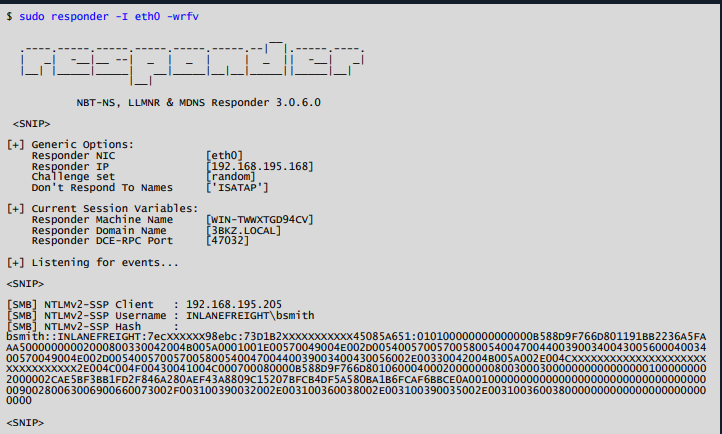
\includegraphics[width=1\linewidth]{initial//evidenceimages/responder.png}
    \caption{Introducir leyenda aquí}
    \label{fig:enter-label}
\end{figure}

\textbf{Descifrado exitoso de un hash de contraseña con Hashcat para revelar el valor en texto claro.}

% Repetimos para LowVulnColor
% Similar estructura que las anteriores tablas.
}
}


\newpage
\section{\iflanguage{spanish}{Apéndices}{Appendices}}
\iflanguage{spanish}
{\subsection{Apéndice A – Gravedad de los Hallazgos}
\qquad Cada hallazgo ha sido clasificado con un nivel de gravedad: crítico, alto, medio o bajo. La clasificación se basa en una evaluación de la prioridad con la que cada hallazgo debe ser considerado y el impacto potencial que puede tener en la confidencialidad, integridad y disponibilidad de los datos de \enterpriseName.

\subsection{Apéndice B – Hosts Explotados}
\subsection{Apéndice C – Usuarios Comprometidos}
\subsection{Apéndice D – Cambios/Limpieza de Hosts}
\subsection{Apéndice E – Revisión de Contraseñas del Dominio \enterpriseName.LOCAL}
}
{\subsection{Appendix A – Finding Severities}
\qquad Each finding has been assigned a severity rating of critical , high, medium, or low. The rating is based off of an assessment of the
priority with which each finding should be viewed and the potential impact each has on the confidentiality, integrity, and
availability of \enterpriseName’s data.
\subsection{Appendix B – Exploited Hosts}
\subsection{Appendix C – Compromised Users}
\subsection{Appendix D – Changes/Host Cleanup}
\subsection{Appendix E – \enterpriseName.LOCAL Domain Password Review}}


%Uncomment this Line
%\section{\iflanguage{spanish}{Fortalezas del Sistema Identificadas}{Identified System Strengths}}
%\iflanguage{spanish}
%{\input{sections/es/system_strengths}}
%{\input{sections/en/system_strengths}}



\newpage
\section{\iflanguage{spanish}{Agradecimientos y Cierre Formal}{Acknowledgments and Formal Closing}}
\iflanguage{spanish}
{{
\qquad Queremos expresar nuestro más sincero agradecimiento a \enterpriseName por su cooperación y apoyo durante el compromiso de prueba de penetración. Su disposición para proporcionar acceso a los sistemas y colaborar con el equipo de pruebas fue crucial para el éxito de esta evaluación. También agradecemos al equipo de TI y a los administradores de sistemas por su colaboración y por facilitar los recursos necesarios para llevar a cabo eficazmente la evaluación.

Este informe presenta los hallazgos de la prueba de penetración, junto con recomendaciones detalladas para mejorar la postura de seguridad. Es importante señalar que la seguridad es un proceso continuo, y recomendamos revisar e implementar las medidas correctivas según las prioridades del negocio.

Agradecemos la oportunidad de haber trabajado en este proyecto y estamos disponibles para cualquier aclaración adicional o para asistir con la implementación de las recomendaciones.
\\

\noindent \textbf{Atentamente,} \\
\brandName \\
\positiones \\
\myName  \\
}

}
{{
\qquad We would like to extend our sincere thanks to \enterpriseName for their cooperation and support throughout the penetration testing engagement. Their willingness to provide access to systems and collaborate with the testing team was crucial to the success of this assessment. We also appreciate the IT team and system administrators for their collaboration and for facilitating the necessary resources to effectively conduct the assessment.

This report presents the findings from the penetration test, along with detailed recommendations to enhance the security posture. It is important to note that security is an ongoing process, and we recommend reviewing and implementing the corrective measures based on the business priorities.

We appreciate the opportunity to have worked on this project and are available for any further clarifications or to assist with the implementation of the recommendations.
\\

\noindent \textbf{Sincerely,} \\
\brandName \\
\position \\
\myName  \\

}

}


\end{document}
